% \section{Reusable Nonlinear Function Unit}\label{sec:method3}


% \subsection{Challenge}
% Exponential function and Sigmoid Linear Unit (SiLU) function are two nonlinear functions in Mamba. 
% Previous methods~\cite{exp_unit,nilsson2014hardware,reggiani2023flex} often design specific unit based on lookup-table or Taylor series approximation to optimize these nonlinear computations.
% However, the optimized nonlinear function unit such exponential function still occupy 30\% of the PE area~\cite{exp_unit,tstc}, leading to much more area overheads.


% \subsection{Motivation and Insights}
% A common approach is to utilize approximation functions to approximate exponential operations, thereby degrading exponential computations to quadratic or even linear operations.
% Using linear approximation methods results in large precision loss ($>$4\% for Mamba-2.8b) while employing higher-order polynomial approximation leads to increased computational overhead.
% We profile the range of these nonlinear functions.
% The input for an exponential function is mostly between -7 and 0, especially for values slightly less than 0,
% while the input range of the SiLU function is from -5 to 4.
% On one hand, we can only approximate nonlinear functions only in these range to concentrate on preventing accuracy loss.
% On the other hand, exponential function and SiLU are similar with element-wise operations except for scaling for each value. 
% Therefore, to avoid increasing area overhead and prevent accuracy loss, our key insight is that \textbf{only by approximating these nonlinear functions in a small range, we can decompose them into several element-wise operations to reuse the reduction alternative PE array architecture in Section~\ref{sec:method1}.}


% \subsection{Approach}

% \textbf{Fast Biased Exponential Algorithm.}
% Given the peculiar distribution observed in the inputs of the exponential function, namely the outer product of $\Delta$ and A, we leverage a set of data points $x=\frac{-7}{n}, n=1,2,...,200$ where the density increases as they approach zero to evaluate the deviation of the approximate calculation from the origin exponential value. Consequently, we modified the fast exp algorithm~\cite{fast_exp} to accommodate specific data ranges and appended a bias at the end to enhance precision and consists of three main steps:

% \begin{enumerate}
%     \item The input \( x \) is linearly transformed into \( x' \).
%     \item \( x' \) is multiplied by $2^{23}$ then cast to an unsigned integer.
%     \item View the x as float-point number and add the bias \( c \).
% \end{enumerate}
%  The fast exp algorithm aims to put $\frac{x}{ln2}$ into exponential bit of $e^{x}$ so that $e^{x} = 2^{\left(\frac{x}{ln2}\right)}$. Float data does not have a direct intuitive representation like unsigned integers, hence cannot be directly used as the exponent bits for $e^{x}$; therefore, conversion to uint is necessary. Additionally, a bias is required to compensate for conversion loss. The exponent of a float is typically subtracted by 127 during actual computations so we also need consider that. Now we can determine the coefficient \(a = \frac{1}{\ln(2)}\) and the term \(b = 127 + bias\), while \(c\) serves as the final bias, effectively reducing the average loss caused by specific data distributions.

% \begin{figure}[!t]
%     \centering
%     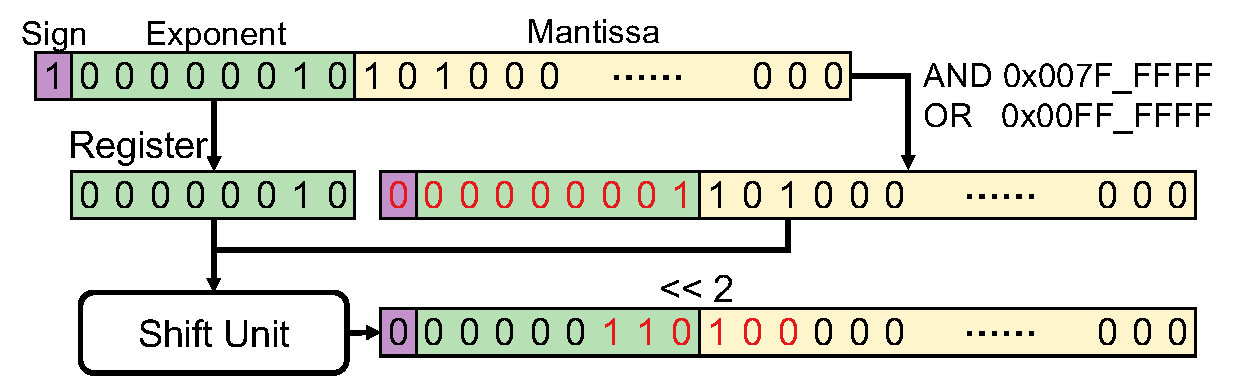
\includegraphics[width=0.48\textwidth]{figures/method3/exp_cast_unit.pdf}
%     \vspace{-20pt}
%     \caption{Hardware implementation of exponential shift unit for our fast exponential approximation.}
%     \vspace{-18pt}
%     \label{fig:approximation}
% \end{figure}

% % \subsection{Approach: SiLU Approximation}
% \textbf{Piecewise SiLU Algorithm.}
% The computational formula for the SiLU function is $SiLU(x) = x\cdot \sigma(x) = \frac{x}{1 + e^{-x}}$
% which involves not only exponentiation but also division operations. Though employing the fast exp algorithm for approximation yields excellent precision, it introduces overhead due to the need for dividers, consequently impacting performance. Our preliminary profiling results indicate that the inputs to the SiLU function are mostly concentrated in the range [-5, 4]. Therefore, we propose segmenting the SiLU function within this interval for approximation. Increasing the number of segments enhances precision but also introduces more conditional branches, thus impacting performance. Consequently, we strike a balance between precision and performance and utilize a 4-segment piecewise function to approximate the SiLU function which is expressed by equation \ref{eq:silu_approx}: Within each interval, further piece-wise approximation is performed based on the distribution of the data.

% \begin{equation}\label{eq:silu_approx}
% f(x) = \left\{
% \begin{aligned}
%     &-0.0135, && \text{if } x < -5 \\
%     &-0.06244x - 0.3457, && \text{if } -5 \leq x < -1.5 \\
%     &0.232(x + 1.181)^{2} - 0.275, && \text{if } -1.5 \leq x \leq 0.75 \\
%     &1.05x - 0.2781, && \text{if } x > 0.75
% \end{aligned}
% \right.
% \end{equation}

% % \subsection{Approach: Hardware Implementation}
% \textbf{Reusable Nonlinear Function Unit.}
% Based on two algorithms for nonlinear functions, we decompose the exponential function into element-wise operations and an shift operation, and SiLU into a range detection and element-wise operations.
% Therefore, we only add a few logics and resue PE arrays to support nonlinear  functions.

% \textit{\underline{As Exponential Function Unit.}} The original computation process of fast exp is overly complex, particularly the float-to-uint conversion unit incurring significant overhead, we have devised a dedicated conversion unit shown in Figure \ref{fig:approximation} for fast exp. Within this unit, the input \( x \) undergoes floating-point linear computation, resulting in \( x' \). Subsequently, we extract the 8 exponent bits of \( x' \), directly representing the required shift length—positive for left shifts and negative for right shifts. Next, employing logical operations, we convert the original floating-point number into the actual representation of the mantissa. Finally, the result is fed into a shift unit and adjusted through a bias unit to yield the output. Due to the ability to simplify the series of linear transformations applied to the input into a single linear transformation, the actual computation only requires 4 cycles.
% % \item 

% \textit{\underline{As SiLU Unit.}} The SiLU unit introduces a range detector in the PE unit, responsible for determining the input's interval and executing the corresponding computation. Due to the most complex operation being quadratic, the actual computational overhead is minimal.
% % \end{itemize}

% % By employing the approximation algorithm, We can eliminate the exponential units and divider within the PE, replacing them with an efficient linear computation flow.